\documentclass[twocolumn,11pt]{jsarticle}
\usepackage{hi_summary}
\usepackage[dvipdfmx]{graphicx,color}
\usepackage{url}
\usepackage{setspace}
\usepackage[top=25truemm,bottom=20truemm,left=20truemm,right=20truemm,columnsep=15pt]{geometry}

\usepackage{dblfloatfix}
\usepackage{enumitem}
\usepackage{booktabs}
\newcommand\doubleRule{\toprule\toprule}
\usepackage{multirow}
\usepackage{caption} 
\captionsetup[table]{skip=1pt}
\setlength{\textfloatsep}{10pt}
\setlength\intextsep{\glueexpr\intextsep/3\relax}

\pagestyle{empty}
\setstretch{0.9}  %% 行間調整

%% 和文タイトル
\title{機械学習による難読化されたプログラムのステルス評価}
%% 英文タイトル
\etitle{Evaluating the Stealth of Obfuscated Program via Machine Learning}
%% 著者
\author{人間情報システム工学科\ \ \ \ バラタ}
%% 指導教員
\supervisor{神崎 雄一郎 准教授}

%% 英文概要
\abstract{Software obfuscation techniques are widely used to protect security-sensitive codes of a program.
One way to evaluate the quality of these techniques is by evaluating its stealthiness, that is, the degree
to which the transformed protected code can be distinguished from unprotected code. This paper proposes a framework
for evaluating the stealthiness of an obfuscated program through machine learning methods. In the case study, the best
model is able to classify between obfuscated and unobfuscated programs used in the dataset with more than 95\% accuracy.}

\begin{document}
\twocolumn[\maketitle \vspace{1.5zw}]

\section{はじめに}
%悪意のあるエンドユーザが物理的に商用のソフトウエアを所有した場合,逆アセンブラなどを用いて内部のコードを解析すればライセンスキーなどのユーザに知られたくない秘密情報が取得される可能性がある.これを防ぐために,ソフトウエアの機能を保持しながら内部のコードを変形し,解析を困難にするというソフトウエア保護の1つの難読化が広く用いられている.

難読化によって変形されたコードがめずらしい特徴を持つことで攻撃者に目立つ場合,難読化によって保護されている秘密情報の場所が攻撃者に知られやすくなり,難読化の効果の低下につながる.そのため,難読化されたプログラムのステルス(\textit{stealth}),すなわち,保護されていないコードとの区別のつきにくさを評価する方法は重要である.

本研究では,ステルスを評価する方法の1つとして,機械学習の分類の手法を用いて「プログラムが難読化されているかどうか」を判定するモデルを構築するフレームワークを提案する.構築したモデルによって難読化されていないと判定される難読化されたプログラムは,ステルスが高いと考える.ケーススタディでは,既存の難読化方法を用いてモデルを構築し,提案方法の有用性について確認する.

\section{アプローチ}
本研究のフレームワークの概要を図~\ref{fig:framework}に示す.この図では,使用したツールを四角形で,ツールの入出力(プログラムやデータ)を楕円で表す.まず,難読化されていないプログラム(ノーマルプログラム)を用意して,難読化ツールによってコードの変形を行う(Step 1).次に,難読化されたプログラムとノーマルプログラムをプログラムの特徴を取り出すツールに与えて,機械学習のための学習データを取得する(Step 2).本研究では,逆アセンブラであるIDA\footnote{IDA: \url{https://www.hex-rays.com/products/ida/}}などのツールに加えて,確率的言語モデルに基づいたコードの不自然さ~\cite{code-art}の数値化方法を用いてプログラムの特徴を取得する.一定のルールに従ってコードを変形する以上,各難読化手法には,論理的に何らかの判定できる特徴を生成する~\cite{pinpoint}ため,機械学習によってデータを分類できると考える.最後のステップ(Step 3)では,機械学習のアルゴリズムを使用して判定モデルを構築する.

\begin{figure}[!t]
 \centering
 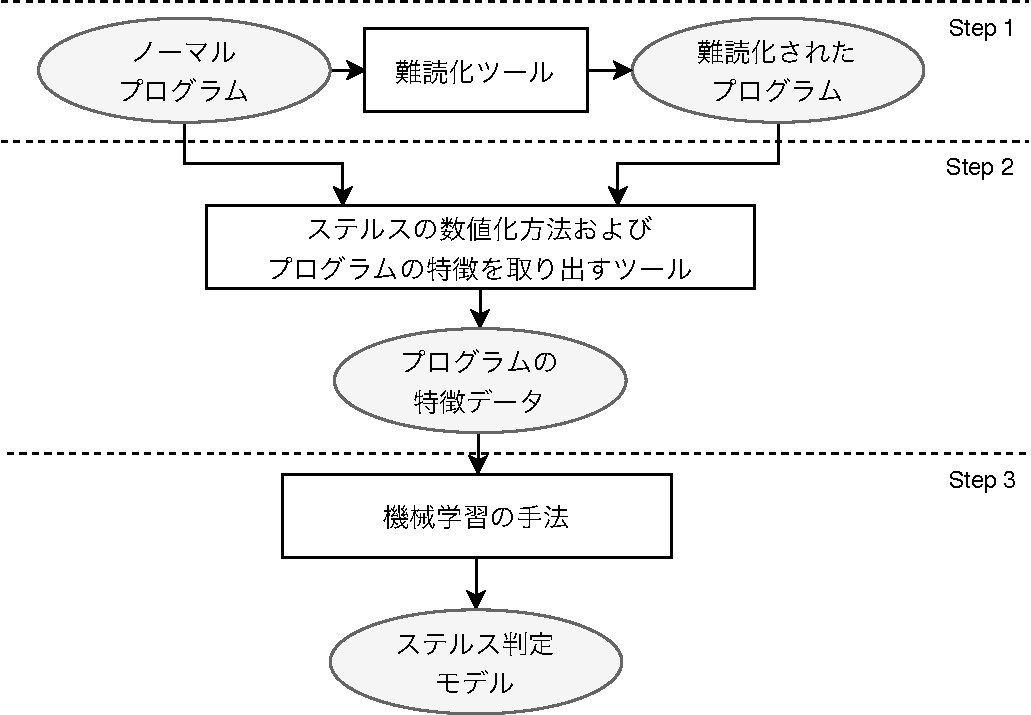
\includegraphics[width=7.5cm]{framework.pdf}
 \caption{提案フレームワークの概要}
 \label{fig:framework}
\end{figure}

\section{ケーススタディ}
\subsection{モデルの構築}
提案フレームワークに沿った判定モデルを実際に構築し,難読化されたプログラムを判定できるかどうかについて調べるケーススタディを行う.

\def\thesubsubsection{(Step \arabic{subsubsection})}
\subsubsection{モデル構築に用いるプログラム} \label{data}
まず,ノーマルプログラムとして,次のものを用意した.

\begin{enumerate}[label={(\arabic*)}]
  \item CentOS\footnote{CentOS: \url{https://www.centos.org/}}のシステムに分類される多様な460個のプログラム.
  \item Tigress\footnote{Tigress: \url{http://tigress.cs.arizona.edu/}}の\texttt{RandomFuns}変形オプションを使用して生成した288個のプログラム.これらは難読化後の動作確認がしやすく,保護すべきコードを含む.\label{orig} 
  \item \ref{orig}の一部を分割した288個のプログラム.
\end{enumerate}

また,難読化されたプログラムは,\ref{orig}をTigressによる難読化及び命令のカムフラージュ法の7つの方法を用いて難読化したもの($288個\times7$)とした.

\subsubsection{プログラムの特徴データ} \label{metrics}
\ref{data}で準備したプログラムをIDAで逆アセンブルし,以下のような関数単位のメトリクスを用いて,プログラムの特徴データを取得する.

\begin{enumerate}
  \item \textbf{Art}: 関数を構成するコード全体の不自然さ~\cite{code-art}の指標である.
  \item \textbf{Max}: コードを3-gram分割したときの関数の最大の「驚き値」~\cite{pinpoint}である.
  \item \textbf{OT}: 3-gramでコードを分割して得られるコード片のうち,驚き値が定められた閾値を超えた関数内のコード片の数である.
  \item \textbf{Len}: 関数に含まれる命令の総数である.
  \item \textbf{Unq}: 関数内のユニークな命令の数である.
\end{enumerate}

\subsubsection{機械学習モデル} \label{model}
\ref{metrics}で取得したプログラムの特徴データを用いて,モデルを構築する.モデルの構築では,Python\footnote{\url{https://www.python.org/}}の機械学習パッケージであるscikit-learn\footnote{\url{http://scikit-learn.org/stable/}}を使用した.

\begin{figure}[!b]
 \centering
 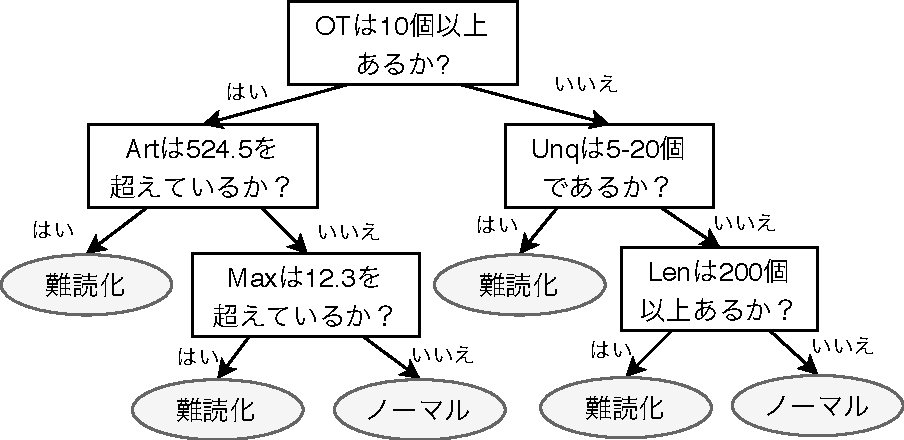
\includegraphics[width=7.5cm]{DT.pdf}
 \caption{本実験での決定木のイメージ}
 \label{fig:DT}
\end{figure}

Breimanによって提案された決定木を拡張したランダムフォレスト~\cite{RF}アルゴリズムを用いて,分類するモデルを構築する.決定木でのプログラムが難読化されたかされていないかの2クラスを分類のイメージを図~\ref{fig:DT}に示す.訓練データのメトリクスをもとに,訓練データラベルを推測することによって,質問の条件を決定し,木構造の一連の質問を学習する.本実験では10本の決定木によって学習を行った.また,2クラスの分類問題に加え,7種類の難読化の各クラスとノーマルクラスの計8クラスを分類するモデルを構築した.

\subsection{モデルの評価結果}

学習モデルの妥当性を確認するために,10分割交差検証,および,テストデータでの検証を行った.表~\ref{table:result}に,正解率(\textit{accuracy})による2クラスと8クラスのモデルの評価結果を示す.CFは10分割交差検証,Valはテストデータの正解率を示している.

\begin{table}[!h]
\centering
\caption{分類モデルの評価結果}
\label{table:result}
\begin{tabular}{c|c|c}
\doubleRule
& 2クラス & 8クラス \\\hline
CF & 96.31\% & 96.23\% \\
Val & 96.48\% & 96.41\% \\
\bottomrule
\end{tabular}
\end{table}

%2クラス分類と同様の方法で,7種類の難読化の各クラスとノーマルクラスの計8クラスを分類するモデルを構築した.モデルの評価結果を表~\ref{table:8class}に示す.

2クラス分類モデルにより,難読化された・されていないの判定は可能であることが分かった.また,難読化法による8クラス分類モデルにより,分岐命令をカムフラージュする難読化~\cite{jmp-obf}などのステルスが高いと思われる難読化法があることが分かった.

\section{おわりに}
本研究では,機械学習によってプログラムが難読化されているかどうかを判定するフレームワークを提案した.このフレームワークを用いた実験においては,最良のモデルでは95\%以上の精度でデータセットにあるプログラムを判定できた.

今後の課題として,難読化方法やメトリクスの種類を増やすことで,さらに有用なステルス評価モデルを検討することが挙げられる.
%今後の課題として,ステルス評価の学習モデルを用いて,複数のコード変形法を組み合わせることによりステルスの高いプログラムを生成する難読化システムの開発が挙げれる.

{\setstretch{0.85}
\begin{thebibliography}{9}

\bibitem{code-art}
Kanzaki, Y., Monden, A., and Collberg, C.
``Code Artificiality: A Metric for the Code Stealth Based on an N-gram Model'',
In \textit{Proc. of the 1st International Workshop on Software Protection} (2015), pp.31-37.

\bibitem{pinpoint}
Kanzaki, Y., Thomborson, C., Monden, A., and Collberg, C.
``Pinpointing and Hiding Suprising Fragments in an Obfuscated Program'',
In \textit{Proc. of the 5th Program Protection and Reverse Engineering Workshop} (2015), PPREW-5, ACM, pp.8:1-8:9.

\bibitem{RF}
Breiman, L.
``Random forests'',
\textit{Machine Learning 45} (2001), 5-32.

\bibitem{jmp-obf}
村上隼之助,神崎雄一郎,門田暁人, 
``分岐命令のカムフラージュに基づくプログラムの制御フローの隠ぺい'',
火の国情報シンポジウム2018,情報処理学会九州支部 (2018).
%Murakami, J., Kanzaki, Y., Monden, A.
%``A Dynamic Obfuscation Method for Hiding Control Flows of the Program'' (2018).

\end{thebibliography}
}

\end{document}
